\documentclass{article}
\usepackage[margin=1in]{geometry}
\usepackage[linesnumbered,ruled,vlined]{algorithm2e}
\usepackage{amsfonts}
\usepackage{amsmath}
\usepackage{amssymb}
\usepackage{amsthm}
\usepackage{enumitem}
\usepackage{fancyhdr}
\usepackage{hyperref}
\usepackage{minted}
\usepackage{multicol}
\usepackage{pdfpages}
\usepackage{standalone}
\usepackage[many]{tcolorbox}
\usepackage{tikz-cd}
\usepackage{transparent}
\usepackage{xcolor}
% \tcbuselibrary{minted}

\author{Nathan Solomon}

\newcommand{\fig}[1]{
    \begin{center}
        \includegraphics[width=\textwidth]{#1}
    \end{center}
}

% Math commands
\renewcommand{\d}{\mathrm{d}}
\DeclareMathOperator{\id}{id}
\DeclareMathOperator{\im}{im}
\DeclareMathOperator{\proj}{proj}
\DeclareMathOperator{\Span}{span}
\DeclareMathOperator{\Tr}{Tr}
\DeclareMathOperator{\tr}{tr}
\DeclareMathOperator{\ad}{ad}
\DeclareMathOperator{\ord}{ord}
%%%%%%%%%%%%%%% \DeclareMathOperator{\sgn}{sgn}
\DeclareMathOperator{\Aut}{Aut}
\DeclareMathOperator{\Inn}{Inn}
\DeclareMathOperator{\Out}{Out}
\DeclareMathOperator{\stab}{stab}

\newcommand{\N}{\ensuremath{\mathbb{N}}}
\newcommand{\Z}{\ensuremath{\mathbb{Z}}}
\newcommand{\Q}{\ensuremath{\mathbb{Q}}}
\newcommand{\R}{\ensuremath{\mathbb{R}}}
\newcommand{\C}{\ensuremath{\mathbb{C}}}
\renewcommand{\H}{\ensuremath{\mathbb{H}}}
\newcommand{\F}{\ensuremath{\mathbb{F}}}

\newcommand{\E}{\ensuremath{\mathbb{E}}}
\renewcommand{\P}{\ensuremath{\mathbb{P}}}

\newcommand{\es}{\ensuremath{\varnothing}}
\newcommand{\inv}{\ensuremath{^{-1}}}
\newcommand{\eps}{\ensuremath{\varepsilon}}
\newcommand{\del}{\ensuremath{\partial}}
\renewcommand{\a}{\ensuremath{\alpha}}

\newcommand{\abs}[1]{\ensuremath{\left\lvert #1 \right\rvert}}
\newcommand{\norm}[1]{\ensuremath{\left\lVert #1\right\rVert}}
\newcommand{\mean}[1]{\ensuremath{\left\langle #1 \right\rangle}}
\newcommand{\floor}[1]{\ensuremath{\left\lfloor #1 \right\rfloor}}
\newcommand{\ceil}[1]{\ensuremath{\left\lceil #1 \right\rceil}}
\newcommand{\bra}[1]{\ensuremath{\left\langle #1 \right\rvert}}
\newcommand{\ket}[1]{\ensuremath{\left\lvert #1 \right\rangle}}
\newcommand{\braket}[2]{\ensuremath{\left.\left\langle #1\right\vert #2 \right\rangle}}

\newcommand{\catname}[1]{{\normalfont\textbf{#1}}}

\newcommand{\up}{\ensuremath{\uparrow}}
\newcommand{\down}{\ensuremath{\downarrow}}

% Custom environments
\newtheorem{thm}{Theorem}[section]

\definecolor{probBackgroundColor}{RGB}{250,240,240}
\definecolor{probAccentColor}{RGB}{140,40,0}
\newenvironment{prob}{
    \stepcounter{thm}
    \begin{tcolorbox}[
        boxrule=1pt,
        sharp corners,
        colback=probBackgroundColor,
        colframe=probAccentColor,
        borderline west={4pt}{0pt}{probAccentColor},
        breakable
    ]
    \color{probAccentColor}\textbf{Problem \thethm.} \color{black}
} {
    \end{tcolorbox}
}

\definecolor{exampleBackgroundColor}{RGB}{212,232,246}
\newenvironment{example}{
    \stepcounter{thm}
    \begin{tcolorbox}[
      boxrule=1pt,
      sharp corners,
      colback=exampleBackgroundColor,
      breakable
    ]
    \textbf{Example \thethm.}
} {
    \end{tcolorbox}
}

\definecolor{propBackgroundColor}{RGB}{255,245,220}
\definecolor{propAccentColor}{RGB}{150,100,0}
\newenvironment{prop}{
    \stepcounter{thm}
    \begin{tcolorbox}[
        boxrule=1pt,
        sharp corners,
        colback=propBackgroundColor,
        colframe=propAccentColor,
        breakable
    ]
    \color{propAccentColor}\textbf{Proposition \thethm. }\color{black}
} {
    \end{tcolorbox}
}

\definecolor{thmBackgroundColor}{RGB}{235,225,245}
\definecolor{thmAccentColor}{RGB}{50,0,100}
\renewenvironment{thm}{
    \stepcounter{thm}
    \begin{tcolorbox}[
        boxrule=1pt,
        sharp corners,
        colback=thmBackgroundColor,
        colframe=thmAccentColor,
        breakable
    ]
    \color{thmAccentColor}\textbf{Theorem \thethm. }\color{black}
} {
    \end{tcolorbox}
}

\definecolor{corBackgroundColor}{RGB}{240,250,250}
\definecolor{corAccentColor}{RGB}{50,100,100}
\newenvironment{cor}{
    \stepcounter{thm}
    \begin{tcolorbox}[
        enhanced,
        boxrule=0pt,
        frame hidden,
        sharp corners,
        colback=corBackgroundColor,
        borderline west={4pt}{0pt}{corAccentColor},
        breakable
    ]
    \color{corAccentColor}\textbf{Corollary \thethm. }\color{black}
} {
    \end{tcolorbox}
}

\definecolor{lemBackgroundColor}{RGB}{255,245,235}
\definecolor{lemAccentColor}{RGB}{250,125,0}
\newenvironment{lem}{
    \stepcounter{thm}
    \begin{tcolorbox}[
        enhanced,
        boxrule=0pt,
        frame hidden,
        sharp corners,
        colback=lemBackgroundColor,
        borderline west={4pt}{0pt}{lemAccentColor},
        breakable
    ]
    \color{lemAccentColor}\textbf{Lemma \thethm. }\color{black}
} {
    \end{tcolorbox}
}

\definecolor{proofBackgroundColor}{RGB}{255,255,255}
\definecolor{proofAccentColor}{RGB}{80,80,80}
\renewenvironment{proof}{
    \begin{tcolorbox}[
        enhanced,
        boxrule=1pt,
        sharp corners,
        colback=proofBackgroundColor,
        colframe=proofAccentColor,
        borderline west={4pt}{0pt}{proofAccentColor},
        breakable
    ]
    \color{proofAccentColor}\emph{\textbf{Proof. }}\color{black}
} {
    \qed \end{tcolorbox}
}

\definecolor{noteBackgroundColor}{RGB}{240,250,240}
\definecolor{noteAccentColor}{RGB}{30,130,30}
\newenvironment{note}{
    \begin{tcolorbox}[
        enhanced,
        boxrule=0pt,
        frame hidden,
        sharp corners,
        colback=noteBackgroundColor,
        borderline west={4pt}{0pt}{noteAccentColor},
        breakable
    ]
    \color{noteAccentColor}\textbf{Note. }\color{black}
} {
    \end{tcolorbox}
}


\fancyhf{}
\setlength{\headheight}{24pt}

\date{\today}
\title{Physics 180E Homework \#1}

\begin{document}
\maketitle

\begin{prob}
\end{prob}
\begin{enumerate}[label=(\alph*)]
    \item According to the ideal gas law,
        \[ \frac{N}{V} = \frac{P}{kT} = \frac{P}{\left( 300 \si{.K} \right) \left( 1.381 \times 10^{-23} \si{.J/K} \right)} = \frac{P}{4.142 \times 10^{-21} \si{.J}}. \]
        When the pressure is 1 Torr, that works out to
        \[ \frac{N}{V} = \frac{1 \si{.Torr}}{ 4.142 \times 10^{-21} \si{.J}} \cdot \frac{133.32 \si{.Pa}}{\si{Torr}} = 3.219 \times 10^{22} \si{.m^{-3}}. \]
        So at 1 Torr, there are $3.219 \times 10^{22}$ atoms per meter cubed. At 100 mTorr, there are $3.219 \times 10^{21}$ atoms per meter cubed. At 10 mTorr, there are $3.219 \times 10^{20}$ atoms per meter cubed.
    \item The mean free path is $\lambda=1/(N \sigma)$. At 1 Torr, that's
        \[ \lambda = \frac{1}{\left( 3.219 \times 10^{22}\si{.m^{-3}} \right) \left( 10^{-15} \si{.cm^{-2}} \right) } \cdot \frac{10^6 \si{.cm^3}}{\si{m^3}} = \frac{1 \si{.cm}}{32.19} = 0.03106 \si{.cm}. \]
        Using that same formula, the mean free path will be $0.3106\si{.cm}$ at $100 \si{.mTorr}$ and $3.106 \si{.cm}$ at $10 \si{.mTorr}$.
    \item Assuming the argon is an ideal gas, mean speed per atom is
        \[ v = \sqrt{ \frac{8 k T}{\pi m_{Ar}}} = \sqrt{ \frac{8PV}{\pi N m_{Ar}}}. \]
        We calculated in part (a) that $PV/N = 4.142 \times 10^{-21}\si{.J}$, and the mass of an argon atom is $6.63 \times 10^{-26} \si{.kg}$, so no matter what the pressure is,
        \[ v = \sqrt{ \frac{8 \cdot (4.142 \times 10^{-21} \si{.m^2/s^2})}{\pi\cdot(6.63\times10^{-26})}} = 399 \si{.m/s}. \]
        The collision frequency is the mean speed divided by the mean free path, which works out to
        \[ \frac{399\si{.m/s}}{0.0311\si{.cm}} = 1.28\times 10^6 \si{.s^{-1}} \]
        at $1 \si{.Torr}$. Therefore the collision frequency is $1.28\times 10^5$ collisions per second at $100\si{.mTorr}$ and $1.28\times 10^4$ collisions per second at $10\si{.mTorr}$.
    \item My answers to parts (a) and (b) would not change, because for those, I did not use the fact that the gas was argon. But my answer for part (c) would change because collision frequency is proportional to mean velocity, which is inversely proportional to the square root of the atomic mass.
        \par
        Of course, that's assuming the cross section doesn't change. In reality though, if pressure and temperature (which were both given) are held constant, helium should have a lower collisional cross section than argon. That means the mean free path would be larger, but the mean speed would also be larger, so I'm not sure whether the collision frequency would increase or decrease.
\end{enumerate}


\bigskip
\begin{prob}
\end{prob}
\begin{enumerate}[label=(\alph*)]
    \item Since the collisional cross section is the same, and the number density of neutral argon atoms is the same as it was at $100\si{.mTorr}$ in question 1(b), the mean free path of the electron is also $0.3106\si{.cm}$.
    \item The speed of the electron is
        \[ v_e = \sqrt{ \frac{2 \cdot (100\si{.eV})}{m_e}} = 5.93 \times 10^6 \si{.m/s}, \]
        so the collision frequency is
        \[ \frac{v_e}{\lambda} = \frac{5.93 \times 10^6 \si{.m/s}}{0.003106\si{m}} = 1.91\times10^9\si{.s^{-1}}. \]
\end{enumerate}


\bigskip
\begin{prob}
\end{prob}
\begin{enumerate}[label=(\alph*)]
    \item The given formula makes no sense, but the answer is
        \[ \frac{1\si{.eV}}{k_B} = \frac{1\si{.eV}}{1.381 \si{.J/K}} \cdot \frac{1\si{.J}}{6.242\times 10^{18}\si{.eV}} = 11600\si{.K}, \]
        where $k_B$ is the constant used to convert between temperatures and energies.
    \item Room temperature is $300\si{.K}$, so the answer is
        \[ (300\si{.K})(k_B) = \frac{300\si{.K}}{11600\si{.K/eV}}=0.0259\si{.eV}. \]
    \item $1\si{.keV} = 1000 \cdot (11600\si{.K}) = 1.16 \times 10^7\si{.K}$.
    \item $50\si{.keV} = 50000 \cdot (11600\si{.K}) = 5.80 \times 10^8\si{.K}$.
    \item ``Thermal velocity" can have a few different meanings, so I'll guess it means the RMS speed. The electrons form an ideal non-relativistic gas, so the kinetic energy per electron is $ \frac{1}{2} m_e v_{RMS}^2 = \frac{3}{2} k_B T$ (where $T$ is temperature), which means the RMS kinetic energy is
        \[ v_{RMS} = \sqrt{ \frac{3 k_B T}{m_e}} =  \sqrt{ \frac{3\si{.eV}}{m_e}} = \sqrt{ \frac{3\si{.eV}}{0.511\si{.MeV.c^{-2}}}} = 0.00587 c = 1.76 \times 10^6 \si{.m/s}. \]
\end{enumerate}

\bigskip
\begin{prob}
\end{prob}
\begin{center}
\begin{tabular}{ |c|c| } 
 \hline
 Atom type & First ionization potential \\ 
 \hline
 \hline
 \ch{He} & $24.6\si{.eV}$ \\ 
 \ch{Ne} & $21.6\si{.eV}$ \\ 
 \ch{Ar} & $15.8\si{.eV}$ \\ 
 \ch{N} & $14.6\si{.eV}$ \\ 
 \hline
\end{tabular}
\end{center}

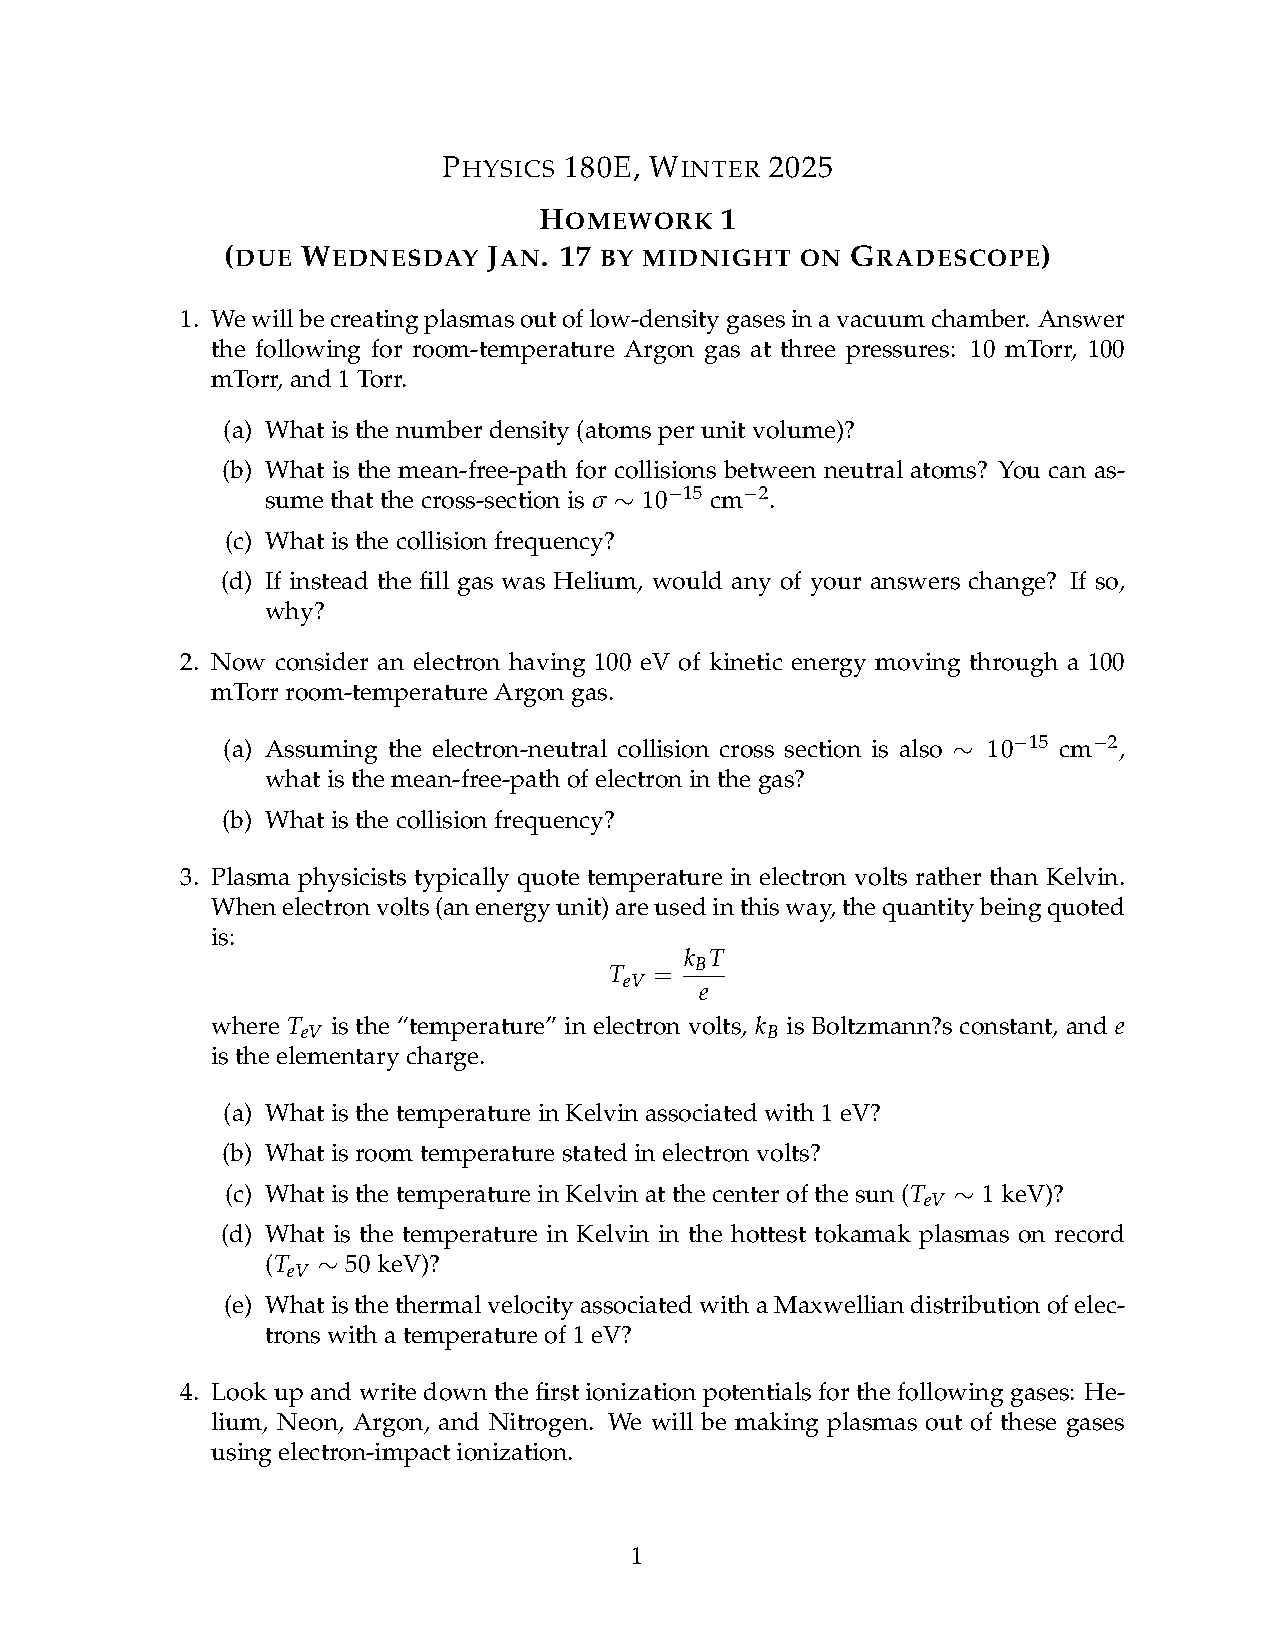
\includepdf[pages=-]{assignment.pdf}

\end{document}
